\documentclass[conference]{IEEEtran}
\usepackage[T1]{fontenc}
\usepackage[utf8]{inputenc}
\usepackage{cite}
\usepackage{amsmath,amssymb,amsfonts}
\usepackage{graphicx}
\usepackage{textcomp}
\usepackage{xcolor}
\usepackage{booktabs}
\usepackage{array}
\usepackage{url}
\graphicspath{{figures/}}
\DeclareUnicodeCharacter{223C}{\ensuremath{\sim}}
\DeclareUnicodeCharacter{2208}{\ensuremath{\in}}
\DeclareUnicodeCharacter{2264}{\ensuremath{\leq}}
\DeclareUnicodeCharacter{2265}{\ensuremath{\geq}}
\DeclareUnicodeCharacter{2286}{\ensuremath{\subseteq}}
\DeclareUnicodeCharacter{2192}{\ensuremath{\to}}
\DeclareUnicodeCharacter{2212}{-}
\DeclareUnicodeCharacter{2203}{\ensuremath{\exists}}
\DeclareUnicodeCharacter{2200}{\ensuremath{\forall}}
\DeclareUnicodeCharacter{2227}{\ensuremath{\wedge}}
\DeclareUnicodeCharacter{2228}{\ensuremath{\vee}}
\DeclareUnicodeCharacter{21D2}{\ensuremath{\Rightarrow}}
\DeclareUnicodeCharacter{2260}{\ensuremath{\neq}}
\DeclareUnicodeCharacter{03A3}{\ensuremath{\Sigma}}
\DeclareUnicodeCharacter{0398}{\ensuremath{\Theta}}
\DeclareUnicodeCharacter{03B8}{\ensuremath{\theta}}
\DeclareUnicodeCharacter{03A0}{\ensuremath{\Pi}}
\DeclareUnicodeCharacter{03C4}{\ensuremath{\tau}}
\DeclareUnicodeCharacter{03C6}{\ensuremath{\varphi}}
\DeclareUnicodeCharacter{03A6}{\ensuremath{\Phi}}
\DeclareUnicodeCharacter{03B2}{\ensuremath{\beta}}
\DeclareUnicodeCharacter{03C1}{\ensuremath{\rho}}
\def\BibTeX{{\rm B\kern-.05em{\sc i\kern-.025em b}\kern-.08em
    T\kern-.1667em\lower.7ex\hbox{E}\kern-.125emX}}
\begin{document}
\title{MPTA-Repair: Multi-Property Clock-Bound Repair for Industrial Timed Automata}
\author{%
% TODO: Add the non-anonymous author names, affiliations, city/country, and email/ORCID. The Markdown-converted draft had an empty \author{} block.
}
\maketitle
\begin{abstract}
Timed automata are widely used to model and verify real-time industrial systems, but practical industrial models often combine multiple components, clocks, synchronizations, guards, invariants, and timing properties. When several properties fail, engineers must identify clock-bound constants that can be repaired without breaking other requirements or changing intended untimed behavior. This paper presents MPTA-Repair, a counterexample-guided workflow for multi-property clock-bound repair of industrial timed automata. MPTA-Repair modifies numerical clock bounds in guards and invariants, uses MaxSMT-based repair generation to synthesize small candidate edits, validates each candidate through full-property regression verification, and applies a TARTAR-style admissibility check for functional equivalence. The workflow jointly considers relations among violated properties, diagnostic traces, and repair variables during iterative refinement.
\end{abstract}
\begin{IEEEkeywords}
Timed automata, multi-property repair, clock-bound repair, industrial systems
\end{IEEEkeywords}
\section{Introduction}
\label{sec:introduction}
Real-time control software is increasingly deployed in domains where
timing faults may directly compromise safety, availability, or mission
success. In railway systems, timed automata have been used to model
train-gate controllers, communication protocols, and railway safety
layers \cite{basile2021unisig}. In automotive and autonomous-driving systems, they have
been used to reason about gear-control logic, road-junction behavior,
and time-bounded decision rules \cite{lindahl1998gear}. In medical cyber-physical
systems, timed models have been used to analyze pacemakers and
ventilator controllers, where physiological timing windows and actuation
deadlines are safety-critical \cite{jiang2012pacemaker}. In aerospace and avionics,
timed-automata models have supported schedulability and deadline
analysis for control software and distributed real-time architectures
\cite{david2010herschel}. Across these domains, correctness depends not only on the
order of discrete events, but also on when these events occur. A
controller that eventually raises an alarm, applies a pulse, sends a
message, or releases a resource may still be incorrect if the action
occurs too early, too late, or for the wrong duration.

Timed automata provide a well-established modeling formalism for this
class of systems \cite{alur1994theory}. Real-time systems are often represented as
networks of timed automata, where clocks, guards, invariants,
synchronizations, and resets describe both discrete behavior and
quantitative timing constraints \cite{bengtsson2004timed}. Verification is then performed
against temporal properties that may include safety, bounded response,
deadline, error-state reachability, alarm-duration, and deadlock-freedom
requirements. When a property is violated, a real-time model checker
such as UPPAAL, Kronos, or opaal can produce a timed diagnostic trace
(TDT), i.e., a timed counterexample that shows how the model reaches a
violating state \cite{daws1996kronos}.

However, diagnosis is only the first step. Interpreting a TDT and
turning it into a correct model edit remains a demanding engineering
task. Realistic control models often contain many locations,
transitions, clocks, guards, invariants, synchronizations, and resets. A
TDT exposes one feasible execution that violates a property, but it does
not directly identify which clock constraint is wrong, whether the
defect lies in a guard or an invariant, or how a bound should be changed
to restore the intended timing behavior \cite{koelbl2019clock}. This ambiguity becomes
more pronounced when the model is checked against multiple properties.
Control-system specifications are usually not single assertions, but
collections of timing requirements that jointly describe safety,
response, scheduling, and reliability obligations \cite{vogel2022patterns}. A local edit
that eliminates one diagnostic trace may still leave related traces
feasible, or may even make another property false. Thus, automated
repair for control models must go beyond explaining a single
counterexample and must validate each candidate repair against the
complete property set.

Existing timed-automata repair techniques provide an important
foundation. Clock-bound repair for timed systems encodes a TDT into
linear real arithmetic, introduces variation variables for clock bounds,
and uses MaxSMT solving to compute small modifications to guards and
invariants \cite{koelbl2019clock}. TarTar extends this idea into an automatic repair
analysis tool that suggests syntactic repairs and checks whether the
repaired model preserves the untimed functional behavior of the original
network timed automaton \cite{koelbl2020tartar}. Other related directions include
parameter synthesis for parametric timed automata \cite{alur1993parametric}, clock-guard
repair through abstraction and testing \cite{andre2019repairing}, robustness analysis for
uncertain timing constants \cite{bendik2021robustness}, and SAT/SMT-based model or program
repair \cite{jose2011bugassist}. These methods show that automated repair of timed
models is feasible, but most existing TDT-based repair workflows remain
centered on one violated property or one diagnostic trace at a time.

The engineering challenge addressed in this paper is different but
complementary to existing single-trace repair and synthesis techniques
\cite{andre2019repairing}. A straightforward repair loop can process one violated
property, collect one TDT, compute a local repair, instantiate a
candidate model, and then run regression verification. This loop is
useful as a baseline, but it may become inefficient or unstable when one
timing fault affects several properties or several related traces.
Similar traces may repeatedly encode overlapping parts of the same
faulty behavior; a candidate that eliminates one trace may still leave
other violations feasible; and a bound changed for one property may
affect another property when the same clock, transition, location, or
synchronization participates in both executions. If all editable bounds
are considered equally plausible repair targets, the solver may explore
many weakly related candidates, including edits that are syntactically
valid but distant from the timing decisions exposed by the observed
violations. Such repairs may pass a local check while giving engineers
little insight into the shared cause of the failures.

This paper presents \textbf{MPTA-Repair}, an automatic repair workflow
for multi-property, multi-counterexample clock-bound repair of
timed-automata control models. Given a faulty model, a set of timing
properties, and diagnostic traces produced by model checking,
MPTA-Repair suggests small modifications to numerical clock bounds in
transition guards and location invariants. The repair space is
intentionally restricted to clock-bound constants, rather than arbitrary
structural edits, specification changes, synchronization changes, or
reset changes. The workflow uses lightweight relation analysis among
properties, diagnostic traces, and editable clock bounds to guide repair
search, but this analysis is only an optimization strategy. Every
accepted candidate must satisfy the complete property set through
regression verification and must pass a TARTAR-style admissibility check
based on functional equivalence. In this way, MPTA-Repair aims to
generate repairs that are not only local counterexample fixes, but also
system-level timing corrections validated against the full set of
control requirements.

We evaluate MPTA-Repair on a suite of control-domain timed-automata
models covering railway alarm control \cite{gonzalez2024realtimedevs}, train-gate control
\cite{behrmann2004tutorial}, automotive gear control, dual-chamber pacemaker control,
autonomous road-junction rules, railway communication timeout handling,
mechanical ventilator control, and aerospace task scheduling. The
evaluation measures repair effectiveness, repair size, runtime,
regression results, and behavior preservation. We compare MPTA-Repair
with an iterative TARTAR-style baseline under the same full-property
regression and admissibility requirements, and report practical
observations from applying automated repair to industrial-style control
models.

This paper makes the following contributions:

\begin{enumerate}
\item
  We formulate clock-bound repair for timed-automata control models as a
  multi-property and multi-counterexample repair problem.
\item
  We present MPTA-Repair, an automatic repair workflow that uses
  diagnostic traces and lightweight relation analysis to guide
  clock-bound repair.
\item
  We implement a prototype repair pipeline combining diagnostic trace
  analysis, MaxSMT-based clock-bound repair, full-property regression
  verification, and TARTAR-style admissibility checking.
\item
  We evaluate the approach on a diverse control-domain benchmark suite
  and compare it with an iterative single-property repair baseline under
  the same acceptance criteria.
\item
  We report practical lessons on applying automated timed-automata
  repair to control models, especially regarding property selection,
  repair interpretability, and the need for full regression after each
  candidate repair.
\end{enumerate}

The remainder of this paper is organized as follows. Section II provides
the background and problem setting, including timed automata, diagnostic
traces, clock-bound repair, and the multi-property repair objective.
Section III presents MPTA-Repair and its relation-guided repair
workflow. Section IV describes the prototype implementation and
evaluation setup. Section V reports the evaluation results and practical
lessons learned from the control-domain models. Section VI discusses
threats to validity and related work. Section VII concludes the paper.

\section{Background and Motivation}
\label{sec:background}

\subsection{Timed Automata and Industrial Networks}

Timed automata provide a standard formal model for systems whose
correctness depends on both discrete control decisions and quantitative
time constraints~\cite{alur1994theory,bengtsson2004timed}. Let $C$ be
a finite set of clocks. A clock constraint over $C$ is a conjunction of
atomic constraints of the form $x \sim b$, where $x \in C$,
$\sim \in \{<,\leq,=,\geq,>\}$, and $b$ is a non-negative numerical
bound. We write $\mathcal{B}(C)$ for the set of such constraints. A
timed automaton is a tuple
\[
  T=(L,\ell_0,C,\Sigma,\Theta,I),
\]
where $L$ is a finite set of locations, $\ell_0 \in L$ is the initial
location, $\Sigma$ is a set of action labels, $\Theta$ is a finite set
of transitions, and $I:L\rightarrow \mathcal{B}(C)$ assigns an invariant
to each location. A transition $\theta \in \Theta$ is written as
\[
  \theta=(\ell,g,a,R,\ell'),
\]
where $\ell$ and $\ell'$ are the source and target locations,
$g\in\mathcal{B}(C)$ is the guard, $a\in\Sigma$ is the action label,
and $R\subseteq C$ is the set of clocks reset by the transition.

The semantics is defined over states $(\ell,u)$, where $\ell$ is a
location and $u:C\rightarrow \mathbb{R}_{\geq 0}$ is a clock valuation.
A delay step lets time elapse in the current location as long as the
location invariant remains satisfied. A discrete step can be taken when
the current clock valuation satisfies the transition guard; the step
moves the automaton to the target location and resets the clocks in
$R$. Thus, guards constrain when discrete actions are enabled, whereas
invariants constrain how long the automaton may remain in a location.

Industrial timed-automata models are usually networks rather than single
automata. A network
\[
  \mathcal{N}=T_1 \parallel \cdots \parallel T_k
\]
composes templates for controllers, plants, environments, communication
protocols, schedulers, and monitors~\cite{larsen1997uppaal}. The exact
product semantics depends on the modeling language and tool, for
example on binary synchronization, broadcast channels, urgent or
committed locations, and data variables. In this work these structural
and data-level features are treated as fixed modeling context. The
repair space is deliberately restricted to numerical clock-bound
occurrences in guards and invariants; synchronization labels, reset
sets, clock references, locations, transitions, data updates, and
property formulas are not repair variables.

This restriction matches a common class of industrial modeling faults.
Timing constants often represent design thresholds, sampling periods,
timeout values, alarm durations, refractory intervals, or scheduling
deadlines. For example, vehicle controllers may need to complete a
gear-shifting sequence within a bounded response time
~\cite{lindahl1998gear}; railway models may encode gate, alarm, or
communication timeout requirements~\cite{basile2021unisig}; medical
devices may encode physiological timing windows~\cite{jiang2012pacemaker};
and avionics or aerospace models may encode execution-time bounds and
deadlines~\cite{han2018avionics}. In such models, an incorrect numerical
bound can make an otherwise intended behavior occur too early, too late,
or for an invalid duration.

We do not assume that all modeling errors are clock-bound errors.
Industrial models may also contain wrong resets, missing transitions,
incorrect synchronizations, erroneous data updates, or incomplete
properties. These faults are outside the current repair space. The
assumption in this paper is narrower: the discrete model structure is
treated as the intended design, while one or more numerical timing
bounds may be inaccurate due to calibration, transcription,
dimensioning, or design-space uncertainty. This is the fault model
targeted by clock-bound repair~\cite{koelbl2019clock} and is consistent
with mutation-based repair and testing, where faults are modeled as
small deviations from an otherwise near-correct artifact~\cite{demillo1978hints}.

\subsection{Properties and Timed Diagnostic Traces}

Timed-automata models are checked against timing properties using
real-time model checkers such as UPPAAL~\cite{larsen1997uppaal}. This
paper focuses on safety-style verification obligations. Direct examples
include queries of the form $A[]\,\psi$, where every reachable state must
satisfy the state predicate $\psi$, and deadlock-freedom checks such as
$A[]\,\mathit{not}\ \mathit{deadlock}$. Bounded-response and deadline
requirements are handled when they are encoded by observer or monitor
templates into safety-style violations, for example by reaching an
error or late location~\cite{vogel2022patterns}. Therefore, the repair
procedure reasons about property violations that can be represented as
reachable safety violations in the instrumented timed-automata network.

A discrete trace skeleton is a finite sequence of transitions
\[
  \tau=\theta_0,\theta_1,\ldots,\theta_{n-1}.
\]
A timed realization of $\tau$ is a sequence of non-negative delays and
clock valuations that makes the transition sequence executable from the
initial state while respecting guards, resets, invariants, and network
synchronization. The skeleton $\tau$ is feasible if it has at least one
timed realization. Given a property $\varphi$, a feasible skeleton is a
timed diagnostic trace (TDT) for $\varphi$ if at least one of its timed
realizations reaches a state that violates the safety condition
associated with $\varphi$~\cite{koelbl2019clock}. Depending on the
model checker, the reported counterexample may contain concrete delays,
symbolic zones, or only enough information to reconstruct the discrete
path and timing constraints.

A TDT is evidence of failure, not a root-cause explanation. It shows that
some timing realization of some discrete behavior violates a property,
but it does not identify which numerical bound is wrong, whether the
fault lies in a guard or invariant, or how the model should be changed.
Several bounds may jointly enable the violating realization, and one
incorrect bound may contribute to several diagnostic traces. Conversely,
blocking the discrete path of a TDT is usually not a valid repair: it
may remove intended functional behavior, such as a request,
acknowledgement, actuation, communication step, or scheduling decision.
A useful repair should change the timing envelope of the behavior while
preserving the relevant untimed functionality of the model.

\subsection{Clock-Bound Repair and Admissibility}

A repairable site is an occurrence of a numerical bound $b$ in an atomic
clock constraint $x\sim b$ that appears in a transition guard or a
location invariant. A clock-bound repair changes this occurrence to a
new value $b'$, equivalently by introducing a variation variable $v$ and
using the repaired bound $b+v$. The comparison operator, clock
reference, transition structure, location structure, synchronization
label, and reset set are kept fixed. Bounds are constrained to remain in
the numerical domain supported by the target model representation.

TDT-based clock-bound repair encodes the feasibility of a diagnostic
trace as constraints over delays and clock values, then introduces
variation variables for the bounds that occur in the encoded guards and
invariants~\cite{koelbl2019clock}. MaxSMT solving can then be used to
prefer small repairs, for example by maximizing soft constraints of the
form $v=0$ and, when needed, minimizing the magnitude of nonzero
variations~\cite{sebastiani2015optimization}. In the single-trace
setting, the resulting candidate is local: the same discrete trace
skeleton should remain feasible, but no feasible realization of that
skeleton should still witness the considered property violation.

Local trace repair is not sufficient for model repair. A bound change
that eliminates one violating realization may create a new violation on
another execution, fail another property, or make intended functionality
unavailable. MPTA-Repair therefore treats MaxSMT-based trace repair as
candidate generation only. A candidate is accepted only after two global
checks. First, the repaired model must satisfy the complete property set
under regression verification. Second, it must pass an admissibility
check based on TARTAR-style functional equivalence~\cite{koelbl2019clock}.

The admissibility check compares untimed functional behavior rather than
timed language equality. This distinction is necessary because a
successful timing repair is expected to remove some violating timed
realizations. Let $\Sigma_f$ denote the functional alphabet used for
admissibility, after excluding monitor-only, observer-only, and internal
labels when appropriate. The intended criterion is
\[
  \mathrm{Untimed}_{\Sigma_f}(M_{\mathit{bad}})
  =
  \mathrm{Untimed}_{\Sigma_f}(M_{\mathit{rep}}),
\]
meaning that the repaired model should not add or remove functional
action traces, although the timing of those traces may change. This
criterion prevents repairs that satisfy safety properties merely by
disabling intended behavior.

\subsection{Why Multi-Property Repair Is Needed}

Industrial timed-automata models are normally validated by a set of
properties rather than by a single assertion~\cite{vogel2022patterns}.
The properties jointly describe the reliability envelope of the model,
including absence of unsafe states, bounded response, timeout handling,
deadline satisfaction, admissible residence times, and deadlock freedom.
Let $M_{\mathit{bad}}$ be a faulty timed-automata network and let
\[
  \Phi=\{\varphi_1,\ldots,\varphi_m\}
\]
be the property set used to validate it. The goal is to construct a
repaired model $M_{\mathit{rep}}$ by changing a small number of
clock-bound constants in guards and invariants such that:
\[
  M_{\mathit{rep}} \models \Phi,
\]
the repaired bounds are well formed, and the repaired model preserves
the projected untimed functional behavior of $M_{\mathit{bad}}$.

The need for joint reasoning can be seen in the gear-shift controller
used as a running example. The driver periodically issues a shift
request, and the controller performs torque cut, gear engagement,
acknowledgement, and recovery. Suppose the faulty controller uses
bounds such as $\mathit{cut}\leq 1$, $\mathit{cut}\geq 1$,
$\mathit{mesh}\leq 3$, and $\mathit{mesh}\geq 3$. One property may
require at least two time units of torque cut before gear engagement,
while another property may require acknowledgement within four time
units of the request. A single-property repair that changes only the
$\mathit{cut}$ bounds from $1$ to $2$ can block the early-engagement
violation. However, if the $\mathit{mesh}$ bounds remain at $3$, the
earliest acknowledgement may occur at time $5$, thereby violating the
response deadline. A multi-property repair must instead consider both
requirements and may need to change both the $\mathit{cut}$ and
$\mathit{mesh}$ timing bounds while preserving the same untimed
request--engage--acknowledge behavior.

This example illustrates why violated properties, diagnostic traces, and
repair variables should not be treated as unrelated subproblems.
Different properties may share clocks, locations, synchronizations, or
execution fragments. Multiple TDTs may expose different realizations of
the same underlying timing defect. Conversely, a repair computed from
one trace can be locally valid yet globally unacceptable after full
regression. MPTA-Repair addresses this setting by accumulating
multi-property and multi-counterexample repair evidence, generating
small clock-bound candidates with MaxSMT, and accepting a candidate only
after complete property regression and functional-admissibility
checking.
\section{Approach}
\label{sec:approach}

\subsection{Overview}

Let $N$ be an NTA and
$\Phi=\{\varphi_1,\ldots,\varphi_m\}$ a set of timed safety
properties. We write $M=(N,\Phi)$ for the repair input.
MPTA-Repair changes only repairable numerical clock bounds in guards
and invariants. It returns a repaired specification
$M'=(N',\Phi)$ only when $N'$ satisfies the accepted-repair condition
in Eq.~\eqref{eq:accepted-repair}; otherwise, it reports that no repair
was found within the resource budget.

The main difficulty is that the properties in $\Phi$ do not define
independent repair tasks. Different properties may constrain the same
clock bound, overlapping execution paths, or different stages of a
shared timing budget. Their TDTs may also have different relations:
some are duplicates, some share only part of a discrete path, and some
reach different violations through the same repairable bounds.
Consequently, an edit derived from one TDT may leave another violating
execution feasible or invalidate a property that already holds. A
single-property workflow that processes these TDTs independently does
not retain their joint constraints and may repeatedly explore
incompatible candidate edits.

MPTA-Repair uses these relations to organize the current repair
problem before MaxSMT solving. At the property level, equivalent or
stronger requirements are identified to avoid redundant constraints.
At the trace level, duplicate and structurally related TDTs are grouped.
At the repair-bound level, each property-trace constraint is mapped to
the bounds that can affect it. Property-trace constraints that depend
on disjoint bound sets form separate search groups, whereas constraints
that share repairable bounds remain in the same group and are solved
jointly. This partition reduces independent parts of the search without
separating constraints that require coordinated edits.

A trace-local repair workflow encodes one TDT, solves a MaxSMT
instance, and validates the resulting candidate. MPTA-Repair extends
this workflow with a shared property-trace pool, relation-guided
selection of active constraints and bounds, and iterative refinement
across properties. At refinement round $k$,
$\mathcal{T}_k$ denotes the current set of property-trace pairs
$(\tau,\varphi)$, where $\tau$ is a TDT for
$\varphi\in\Phi$. The framework verifies $N'$ against the full property
set, updates $\mathcal{T}_k$, constructs a joint MaxSMT problem for the
dependent groups, and instantiates the resulting clock-bound edits in a
candidate model.

A candidate is not accepted merely because it satisfies the active
MaxSMT constraints. It must first pass full-property regression
verification and then the admissibility check based on functional
equivalence. If either check fails, newly exposed TDTs are added to the
pool and the rejected assignment is excluded from later rounds. Only a
candidate that passes both checks is returned as $M'$.
Figure~\ref{fig:mpta-repair-workflow} summarizes this iterative
workflow.

\begin{figure*}[t]
  \centering
  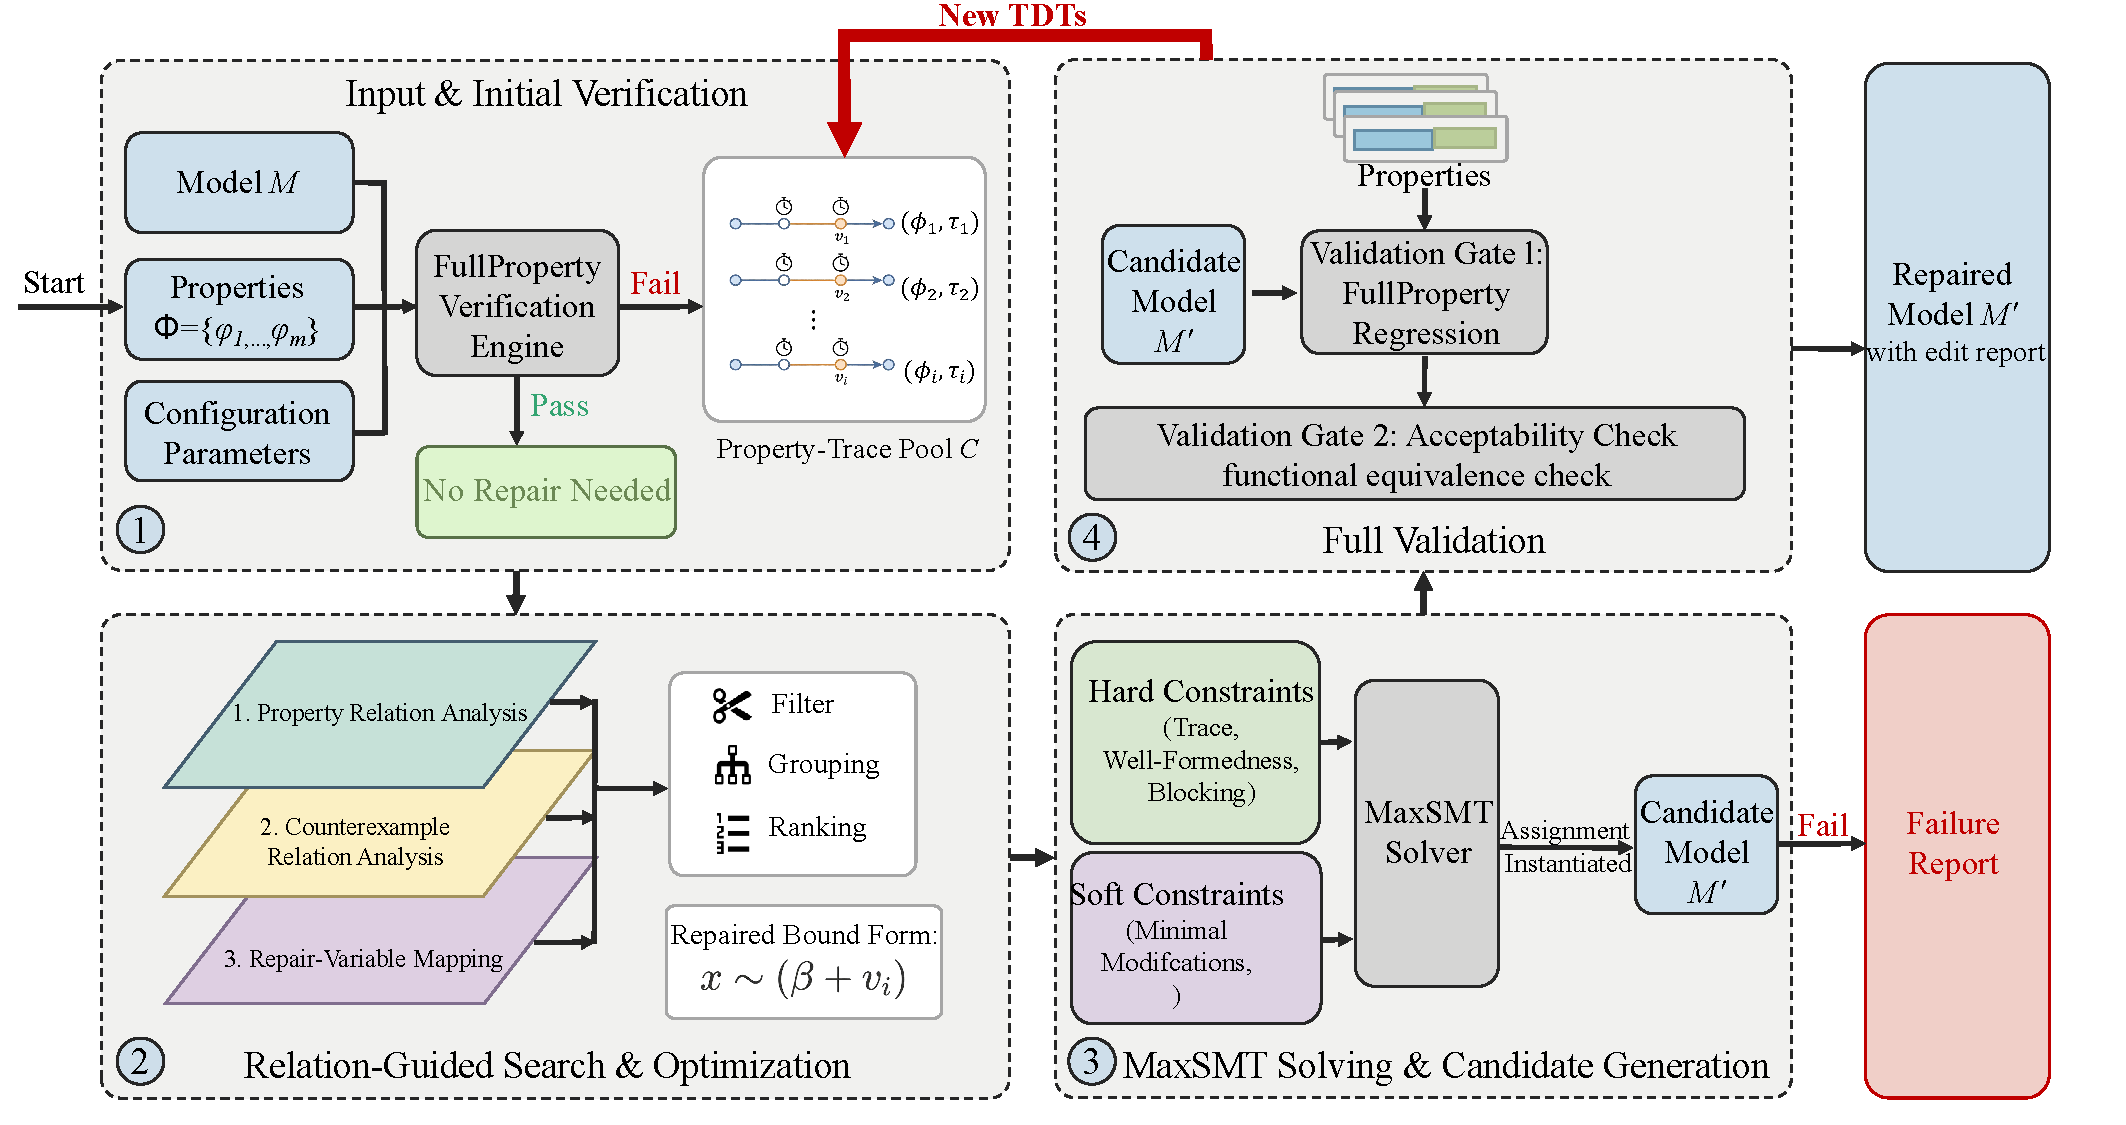
\includegraphics[width=0.86\textwidth]{MPTA_Repair_overview.pdf}
  \caption{Overview of the MPTA-Repair workflow.}
  \label{fig:mpta-repair-workflow}
\end{figure*}

\subsection{Joint Trace Encoding and Optimization Objective}

MPTA-Repair follows the clock-bound variation strategy used in TARTAR
\cite{kolbl2019clock}. Let $S$ denote the set of repairable clock-bound
occurrences. For each occurrence $s\in S$, the original numerical bound
$b_s$ in a transition guard or location invariant is associated with a
variation variable $\delta_s$. This ensures that the repaired constraint
retains the original clock reference and comparison operator while
incorporating a shifted value:
\begin{equation}
  b'_s = b_s + \delta_s
\end{equation}
The repair space is therefore strictly restricted to clock-bound
constants, keeping transition structures and discrete updates unaltered.

MPTA-Repair builds on the trace-encoding formulation of TARTAR and
extends it to the multi-property setting \cite{kolbl2019clock}. Given
a TDT
\begin{equation}
\begin{aligned}
  \tau ={}&
  \ell_0 \xrightarrow{d_0,e_0} \ell_1 \cdots \\
  &{}\xrightarrow{d_{n-1},e_{n-1}} \ell_n
\end{aligned}
\end{equation}
a trace path is encoded as a conjunction of linear arithmetic
constraints:
\begin{equation}
\begin{aligned}
  \operatorname{Path}(\tau,\rho,\mathbf{z}_{\tau})
  ={}& \mathit{Init}(\nu_0)\\
  &{}\land
  \bigwedge_{i=0}^{n-1}\Bigl(
    d_i \ge 0
    \land \mathit{Inv}(\ell_i,\nu_i+d_i,\rho)\\
  &{}\land
    \mathit{Guard}(e_i,\nu_i+d_i,\rho)\\
  &{}\land
    \nu_{i+1}
    =
    \mathit{Reset}(\nu_i+d_i,R_i)
  \Bigr)
\end{aligned}
\end{equation}
Here, $\rho$ denotes the modified bounds, and $\mathbf{z}_{\tau}$
collects the delays and clock valuations. The reset equation
$\nu_{i+1}=\mathit{Reset}(\nu_i+d_i,R_i)$ updates the valuation after
transition $e_i$ by resetting clocks in $R_i$ and preserving the others.
The original violation encoding combines path executability with the
final property violation:
\begin{equation}
  \operatorname{Enc}(\tau,\varphi,\rho)
  =
  \operatorname{Path}(\tau,\rho,\mathbf{z}_{\tau})
  \land
  \mathit{Bad}_{\varphi}(\ell_n,\nu_n)
\end{equation}
The predicate $\mathit{Bad}_{\varphi}(\ell_n,\nu_n)$ characterizes the
violation state of $\varphi$ at the final location. To block this
violating behavior while preserving executability of the discrete path
skeleton, the single-trace repair constraint uses two copies of the
trace variables:
\begin{equation}
\begin{aligned}
  &\Psi_{\tau,\varphi}^{\mathrm{repair}}(\rho)
  =
  \exists \mathbf{z}_{\tau}^{+}.
  \operatorname{Path}(\tau,\rho,\mathbf{z}_{\tau}^{+}) \\
  &\quad{}\land
  \neg \exists \mathbf{z}_{\tau}^{-}.
  \Bigl(
    \operatorname{Path}(\tau,\rho,\mathbf{z}_{\tau}^{-}) \\
  &\qquad{}\land
    \mathit{Bad}_{\varphi}(\ell_n^{-},\nu_n^{-})
  \Bigr)
\end{aligned}
\end{equation}
The first part requires that the original discrete path skeleton still
has at least one timed realization after repair. The second part
requires that no assignment of delays and clock valuations can make that
same path violate $\varphi$.

We extend this single-trace formulation to a joint, multi-property
incremental setting. At refinement round $k$, counterexamples from all
currently violated properties are accumulated into a trace pool
\begin{equation}
  \mathcal{T}_k=\{(\tau_j,\varphi_j)\}_{j=1}^{m_k}
\end{equation}
MPTA-Repair assembles a joint MaxSMT problem with the constraint system
defined as
\begin{equation}
\begin{aligned}
  \mathcal{F}_k(\rho)
  =
  &\mathit{Dom}(\rho)
  \land \mathit{Block}_k(\rho) \\
  &{}\land
  \bigwedge_{(\tau,\varphi)\in \mathit{Select}(\mathcal{T}_k)}
  \Psi_{\tau,\varphi}^{\mathrm{repair}}(\rho)
\end{aligned}
\end{equation}
Here, $\mathit{Dom}(\rho)$ enforces static interval consistency and
domain limits, such as $b'_s\ge 0$, and
$\mathit{Select}(\mathcal{T}_k)$ represents a reduced subset of traces
obtained after relation-aware filtering. When an instantiated candidate
NTA fails verification, the constraint system is updated
incrementally. The framework expands the pool via
\begin{equation}
  \mathcal{T}_{k+1}
  =
  \mathcal{T}_k
  \cup
  \mathit{NewTDTs}(N(\rho_k),\Phi)
\end{equation}
and updates the search-space block to exclude the failed assignment
$\rho_k$ over the set of repairable bounds $S$:
\begin{equation}
  \mathit{Block}_{k+1}(\rho)
  =
  \mathit{Block}_k(\rho)
  \land
  \left(
    \bigvee_{s\in S} \delta_s \ne \delta_s^k
  \right)
\end{equation}
where $\delta_s^k$ is the valuation assigned to variation variable
$\delta_s$ in round $k$.

The optimization objective is governed by a hierarchical set of soft
constraints. MPTA-Repair uses a lexicographic objective that first
favors small repairs and then incorporates risk- and coverage-based
priorities:
\begin{equation}
\operatorname*{lex\,min}_{\rho}
\left(
\begin{aligned}
  &\sum_{s\in S}\mathbf{1}\{\delta_s \ne 0\},\\
  &\sum_{s\in S}|\delta_s|,\\
  &\sum_{s\in S} \mathit{risk}_s \cdot \mathbf{1}\{\delta_s \ne 0\},\\
  &-\sum_{s\in S} \mathit{benefit}_s \cdot \mathbf{1}\{\delta_s \ne 0\}
\end{aligned}
\right)
\end{equation}
Here, $\mathbf{1}\{\cdot\}$ denotes the indicator function, yielding 1
when the inner condition holds and 0 otherwise. The primary and
secondary objectives minimize the number and total magnitude of altered
clock bounds to produce concise repairs. The third term incorporates a
penalty coefficient $\mathit{risk}_s$ to discourage modifications prone
to regression, while the final term uses a reward coefficient
$\mathit{benefit}_s$ to prioritize repair sites that cover a broader set
of violated traces.

\subsection{Relation-Guided Search Optimization}

During refinement, accumulating violated properties, TDTs, and editable
bounds expands the MaxSMT search space. To reduce redundant
constraints, MPTA-Repair uses relation-guided optimization to filter,
group, and rank constraints and repair variables. These heuristics only
guide the search; correctness is still guaranteed through full-property
regression verification and an admissibility check.

At the property layer, timed safety properties are normalized into an
$\mathtt{A}[]$ fragment over location predicates and clock or integer
constraints. Equivalence is detected by the syntactic identity of
normalized forms, while dominance is evaluated under logical
subsumption, e.g., $\mathtt{A}[]\, x \le 5$ subsumes
$\mathtt{A}[]\, x \le 10$ within the same structural context.
MPTA-Repair then retains only the stronger properties for solving to
optimize efficiency.

At the counterexample layer, MPTA-Repair maintains a TDT pool indexed by
violated properties. Exact duplicates are removed, and the remaining
traces are annotated with traversed transitions, visited locations,
active clocks, and guard or invariant bounds. Traces with identical
discrete transition sequences or overlapping clock zones are grouped to
reveal common bottlenecks. A trace constraint is omitted from the active
encoding only when it is an exact duplicate or soundly subsumed by an
encoded trace constraint.

At the repair-bound layer, MPTA-Repair maps each active property-trace
constraint to the clock bounds occurring in or affecting its encoding.
This mapping restricts active MaxSMT decision variables to bounds
relevant to the current counterexample pool and ranks them for candidate
generation. Bounds with higher relational scores are prioritized
because their modifications are more likely to satisfy the joint
constraint system.
\section{Implementation and Experimental Evaluation}
\label{sec:evaluation}

This section details the implementation of the MPTA-Repair framework
and systematically evaluates its practical effectiveness across both
standardized benchmark models and complex industrial case studies. To
clearly distinguish our targeted contribution while maintaining
practical applicability, our methodology strictly focuses on the
automated repair of numerical clock bounds within transition guards and
location invariants, deliberately avoiding arbitrary alterations to the
underlying discrete transition logic. This focused parametric repair
space is pragmatic for industrial contexts, because modifying clock
bounds can correct clerical modeling mistakes and provide useful
insights for redimensioning system time resources without disrupting the
intended functional design. Furthermore, we compare MPTA-Repair with a
specialized iterative baseline technique constructed by extending the
foundational TARTAR repair idea \cite{koelbl2020tartar} with a
sequential repair loop. This comparison demonstrates the necessity of
incorporating multi-property regression and multi-counterexample
analysis to prevent secondary errors during repair.

\subsection{Prototype Implementation}

We implemented MPTA-Repair as a highly integrated, incremental repair
pipeline built around a specialized timed-automata model parser, a
verification interface using UPPAAL \cite{larsen1997uppaal}, a
MaxSMT-based repair backend powered by Z3 \cite{demoura2008z3}, a
dedicated admissibility checker, and an overarching iterative refinement
control loop. Initially, the repair frontend parses the faulty model to
extract editable clock-bound variables embedded within transition guards
and location invariants. The trace analyzer then maps observed
diagnostic traces to these extracted variables. Concurrently, the
relation analyzer establishes dependencies among the specified
properties, generated traces, and localized repair sites in order to
prioritize candidate generation and reduce the computational search
space.

Once the MaxSMT backend synthesizes a viable candidate assignment, the
model writer instantiates the corresponding repaired model. Final
candidate acceptance relies on two consecutive validation gates designed
to guarantee both timing correctness and behavioral fidelity. The first
gate performs full-property regression verification through UPPAAL to
ensure that no collateral property violations occur. The second gate is
an admissibility check for functional equivalence following the
TARTAR-style criterion \cite{koelbl2019clock}. This module constructs
untimed automata from both the original and repaired models and performs
a comparative language-equivalence test. The system rejects any
candidate that inadvertently adds or removes functional untimed
behavior. Whenever either validation gate rejects a candidate, the
control loop captures the newly exposed diagnostic traces and feeds them
back into the relation analyzer. This initiates an incremental,
counterexample-guided refinement iteration that further constrains the
MaxSMT solver with updated evidence until a globally correct and
admissible repair is found or the search budget is exhausted.

\subsection{Evaluation Strategy and Datasets}

We evaluate the proposed framework on two dataset groups. The benchmark
dataset consists of timed-automata models collected from UPPAAL and XTA
benchmark sources. These models provide structural diversity and allow
comparison with existing clock-bound repair settings. The industry
dataset contains practical case studies involving railway alarm and
communication scenarios
\cite{gonzalez2024realtimedevs,basile2021unisig}, train-gate behavior
\cite{behrmann2004tutorial}, automotive gear control
\cite{lindahl1998gear}, cardiac pacing \cite{jiang2012pacemaker},
autonomous road-junction rules \cite{belguidoum2021junction},
mechanical ventilation \cite{cuartas2023ventilator}, and aerospace
scheduling \cite{david2010herschel}. Together, the two dataset groups
test both algorithmic behavior on established examples and practical
behavior on industrial models with synchronization, multiple
components, and domain-level timing requirements.

Because naturally occurring faulty timed-automata models are scarce, we
use a mutation-based evaluation strategy \cite{jia2011mutation}. Faults
are seeded into verified reference models by modifying clock-bound
constants in guards and invariants. For simple mutants, one bound is
changed and the resulting model is retained if it violates at least one
selected timing safety property. For complex mutants, multiple
clock-bound edits are injected to simulate interacting timing faults.
Generated mutants are filtered to remove invalid or trivial cases: each
retained mutant must be syntactically valid and must violate at least
one selected property.

We compare MPTA-Repair with an adapted iterative TARTAR-style baseline
\cite{koelbl2020tartar}. For fairness, the baseline receives the same
full-property regression and admissibility validation gates used by
MPTA-Repair. However, the baseline generates repairs from one violated
property or diagnostic trace at a time. It does not jointly analyze
relations among multiple properties, counterexamples, and repair
variables before candidate generation. This difference allows us to
measure the benefit of the multi-property and multi-counterexample
repair strategy.

\subsection{Experimental Results}

The experimental results show that MPTA-Repair outperforms the
iterative baseline, particularly on complex industrial models. On the
benchmark dataset, the baseline repairs 72\% of the cases, while
MPTA-Repair repairs 93\%. On the industry dataset, the gap is larger:
the baseline repairs 20\% of the cases, while MPTA-Repair repairs
76\%. These results suggest that the proposed workflow remains
effective on established timed-automata benchmarks and is more robust
when properties and traces interact in industrial models.

\begin{table}[t]
\caption{Overall repair outcomes reported in the source draft.}
\label{tab:overall-results}
\centering
\scriptsize
\setlength{\tabcolsep}{2pt}
\begin{tabular}{@{}p{0.24\columnwidth}p{0.34\columnwidth}p{0.09\columnwidth}p{0.11\columnwidth}p{0.13\columnwidth}@{}}
\toprule
Dataset group & Method & Cases & Repaired & Success rate \\
\midrule
Benchmark & Iterative TARTAR-style baseline & N1 & R1 & 72\% \\
Benchmark & MPTA-Repair & N1 & R2 & 93\% \\
Industry & Iterative TARTAR-style baseline & N2 & R3 & 20\% \\
Industry & MPTA-Repair & N2 & R4 & 76\% \\
\bottomrule
\end{tabular}
% TODO: Replace placeholder counts N1, N2, R1, R2, R3, and R4 with final evaluated counts, and confirm the success rates.
\end{table}


The baseline remains competitive on simpler benchmark models where
faults are highly localized. In such cases, a single diagnostic trace
often provides enough evidence to infer a useful clock-bound edit.
However, in industrial models with interacting concurrent components,
synchronization mechanisms, and observer templates, local baseline
repairs frequently fail later global validation checks.

Our analysis identifies two main reasons for the stronger performance
of MPTA-Repair. First, multi-counterexample accumulation reduces
overfitting to one timed diagnostic trace. A single trace usually
exposes only one timing realization of a deeper fault, so a candidate
that eliminates that trace may still leave related violations feasible.
By accumulating diagnostic traces from multiple operational modes,
MPTA-Repair can synthesize small joint edit sets that address the shared
timing fault without requiring excessive refinement rounds.

Second, relation-guided optimization improves search efficiency and
candidate quality. Property relations help avoid repeatedly solving
equivalent obligations. Counterexample relations identify traces that
share path fragments or repair variables. Repair-variable relations
focus the solver on clock bounds close to the observed violations
rather than opening all syntactically editable bounds in the model. In
the ablation analysis, removing relation guidance increased the number
of generated candidates and the frequency of regression failures.
Successful repairs typically modified only one or two clock bounds, and
the average edit magnitude remained close to the injected fault size,
which makes the suggested repairs easier for engineers to inspect.

\subsection{Discussion and Practical Lessons}

The evaluation highlights several practical lessons for applying
automated repair to industrial timed automata. First, full-property
regression testing is necessary. Industrial properties are often
interdependent: a local fix that satisfies a response monitor can
violate a separate safety monitor that constrains maximum waiting time.
MPTA-Repair avoids accepting such regressions by treating restoration of
the full property set as a global objective rather than as a sequence of
isolated local patches.

Second, admissibility changes the meaning of repair success. Without
checking functional equivalence, a solver could satisfy a timed property
by disabling intended behavior, for example by blocking a necessary
communication response or preventing a critical action. Such a candidate
may eliminate the observed timed diagnostic trace, but it is not a valid
repair for an industrial model. The admissibility check therefore
prevents property satisfaction from being achieved through unacceptable
loss of untimed behavior.

Finally, the unrepaired cases show the limits of the current repair
space. Some attempts fail because of solver, verification, or
admissibility timeouts, and some models use syntax outside the supported
fragment. Other cases appear to lack a feasible repair within numerical
clock-bound edits alone. These failures suggest that broader repair
actions, such as changing synchronization labels, clock resets, or
discrete data updates, are an important direction for future work.

\input{sections/discussion}
\input{sections/related_work}
\section{Conclusion}
\label{sec:conclusion}
This paper presented \textbf{MPTA-Repair}, an automatic repair workflow
for multi-property, multi-counterexample clock-bound repair of
timed-automata control models. The method addresses a practical
limitation of local TDT-based repair: control models are commonly
validated against multiple timing properties, and one timing defect may
produce several related counterexamples. Repairing one trace in
isolation may therefore be insufficient.

MPTA-Repair collects diagnostic traces from violated properties, uses
lightweight relations among properties, traces, and repairable bounds to
guide repair search, and synthesizes small clock-bound edits using a
MaxSMT-based backend. Every candidate is validated by full-property
regression and a TARTAR-style admissibility check based on functional
equivalence \cite{koelbl2019clock}. This design ensures that accepted repairs are not
merely local counterexample fixes, but system-level timing corrections
that preserve intended behavior.

Our evaluation on non-control and control-domain timed-automata
benchmarks shows that MPTA-Repair improves repair success over an
iterative TARTAR-style baseline, especially on control-domain models
where multi-property interaction and admissibility constraints are
prominent. The results also show that failures remain meaningful:
unrepaired cases often require changes outside the clock-bound repair
space or exceed the configured solving and validation budgets.

Future work will extend the repair space beyond numerical clock bounds
to include resets, clock references, synchronization labels, and
structural edits. We also plan to strengthen counterexample generation,
improve relation-guided decomposition, and evaluate the method on larger
industrial timed-automata models.

\bibliographystyle{IEEEtran}
\bibliography{refs}
\end{document}
